%
% Niniejszy plik stanowi przykład formatowania pracy magisterskiej na
% Wydziale MIM UW.  Szkielet użytych poleceń można wykorzystywać do
% woli, np. formatujac wlasna prace.
%
% Zawartosc merytoryczna stanowi oryginalnosiagniecie
% naukowosciowe Marcina Wolinskiego.  Wszelkie prawa zastrzeżone.
%
% Copyright (c) 2001 by Marcin Woliński <M.Wolinski@gust.org.pl>
% Poprawki spowodowane zmianami przepisów - Marcin Szczuka, 1.10.2004
% Poprawki spowodowane zmianami przepisow i ujednolicenie 
% - Seweryn Karłowicz, 05.05.2006
% Dodanie wielu autorów i tłumaczenia na angielski - Kuba Pochrybniak, 29.11.2016

% dodaj opcję [licencjacka] dla pracy licencjackiej
% dodaj opcję [en] dla wersji angielskiej (mogą być obie: [licencjacka,en])
\documentclass[licencjacka]{pracamgr}
\usepackage{amsfonts}
\usepackage{datetime}
\usepackage{mathtools}
\usepackage{amsthm}
\usepackage{lipsum}
\usepackage[upright]{fourier} 
\usepackage[usenames,dvipsnames]{xcolor}
\usepackage{tkz-euclide} 
\usetkzobj{all}
\usetikzlibrary{calc}
\definecolor{fondpaille}{cmyk}{0,0,0.1,0}

\DeclarePairedDelimiter\ceil{\lceil}{\rceil}
\DeclarePairedDelimiter\floor{\lfloor}{\rfloor}

\newcommand{\defeq}{\vcentcolon=}


% Dane magistranta:
\autor{Filip Plata}{371335}

\title{Prezentacja Dehna}

%\tytulang{An implementation of a difference blabalizer based on the theory of $\sigma$ -- $\rho$ phetors}

%kierunek: 
% - matematyka, informacyka, ...
% - Mathematics, Computer Science, ...
\kierunek{matematyka}

% informatyka - nie okreslamy zakresu (opcja zakomentowana)
% matematyka - zakres moze pozostac nieokreslony,
% a jesli ma byc okreslony dla pracy mgr,
% to przyjmuje jedna z wartosci:
% {metod matematycznych w finansach}
% {metod matematycznych w ubezpieczeniach}
% {matematyki stosowanej}
% {nauczania matematyki}
% Dla pracy licencjackiej mamy natomiast
% mozliwosc wpisania takiej wartosci zakresu:
% {Jednoczesnych Studiow Ekonomiczno--Matematycznych}

% \zakres{Tu wpisac, jesli trzeba, jedna z opcji podanych wyzej}

% Praca wykonana pod kierunkiem:
% (podać tytuł/stopień imię i nazwisko opiekuna
% Instytut
% ew. Wydział ew. Uczelnia (jeżeli nie MIM UW))
\opiekun{prof. dr. hab. Sławomir Nowak}

% miesiąc i~rok:
\date{Maj 2019}

%Podać dziedzinę wg klasyfikacji Socrates-Erasmus:
\dziedzina{ 
%11.0 Matematyka, Informatyka:\\ 
11.1 Matematyka\\ 
%11.2 Statystyka\\ 
%11.3 Informatyka\\ 
%11.4 Sztuczna inteligencja\\ 
%11.5 Nauki aktuarialne\\
%11.9 Inne nauki matematyczne i informatyczne
}

%Klasyfikacja tematyczna wedlug AMS (matematyka) lub ACM (informatyka)
\klasyfikacja{20F06}

% Słowa kluczowe:
\keywords{Prezentacja Dehna, problem słów, zbiór isoperymetryczny, grupa hiperboliczna}

% Tu jest dobre miejsce na Twoje własne makra i~środowiska:
\newtheorem{defi}{Definicja}[section]
\newtheorem{exampl}{Przykład}[section]
\newtheorem{ther}{Twierdzenie}[section]
\newtheorem{lemma}{Lemat}[section]
\newtheorem{stmt}{Stwierdzenie}[section]

% koniec definicji

\begin{document}

\maketitle

%tu idzie streszczenie na strone poczatkowa
\begin{abstract}

Zebranie i prezentacja klasycznych wyników z dziedziny problemu słów i geometrii hiperbolicznej. Zawiera przetłumaczony i uzupełniony dowód twierdzenia o istnieniu przerwy isoperymetrycznej, na podstawie pracy \cite{bib:subquadratic_isoperimetric_inequality}.

\end{abstract}

\tableofcontents
%\listoffigures
%\listoftables


\chapter*{Wstęp}
\addcontentsline{toc}{chapter}{Wstęp}

Problem słów naturalnie pojawia się w informatyce teoretycznej. Mając dane dwa słowa oraz zbiór słów zwanych relatorami, chcemy uzyskać z pierwszego słowa drugie poprzez wstawianie relatorów w dowolne miejsce oraz skracanie podsłów postaci $uu^{-1}$.

Przyjrzymy się, jak podstawowe narzędzia teorii grup oraz geometrii hiperbolicznej Gromova prowadzą do charakteryzacji grup, w których problem słów jest możliwy do rozwiązania w efektywny sposób. Pokażemy, jak można uzyskać charakteryzację grup hiperbolicznych jako jedynych grup z podkwadratową funkcją Dehna.

Wkładem autora jest uściślenie zawartych rozumowań, przede wszystkim charakteryzacji grup hiperbolicznych przez podkwadratową funkcję Dehna. Dowód został doprecyzowany oraz przepisany w sposób zdaniem autora prostszy do zrozumienia. Szczególnie istotne autorowi wydawało się precyzyjne sformalizowanie kroków dowodu, które opierają się na intuicjach geometrycznych. Zdaniem autora są to miejsca, w których najłatwiej o nieścisłości.

Ujęcie i sposób zapisania dowodu umożliwia też jego łatwiejsze zrozumienie również dla czytelników mniej zaznajomionych z tematyką problemu słów. W tej pracy zostały zebrane wszystkie wykorzystywane narzędzia matematyczne, poza ścisłym opisem diagramów van Kampena.

Oprócz tego, w jednym z lematów - \ref{lemma:olshanskii_3} - dzięki uważnemu przyjrzeniu się dowodowi, została poprawiona stała w jednej z nierówności.

\chapter{Problem słów a teoria grup}\label{r:concepts}

\section{Definicje}

Zaczniemy od wprowadzenia pojęć z teorii grup oraz podstawowe słownictwo związane z napisami.

\begin{defi}\label{strings}
Niech $n \in \mathbb{N}$, zbiór $A = \{ a_i : 1 \leq i \leq n, i \in \mathbb{N} \}$ nazwiemy alfabetem, natomiast $a_i$ nazwiemy literami. Słowem bądź napisem nazwiemy uporządkowany, skończony ciąg liter. Będziemy je oznaczać poprzez wypisywanie liter bezpośrednio obok siebie. Mówimy, że ciąg jest słowem nad alfabetem A, jeśli wszystkie jego elementy należą do A.

Będziemy również rozważać słowo puste, tj. pusty ciąg liter. Będziemy je dla każdego alfabetu oznaczać poprzez $\ \epsilon$.
\end{defi}

\begin{exampl}\label{string_binary}
Bardzo istotnym alfabetem w wielu zastosowaniach jest alfabet binarny $A = \{ 0, 1 \}$. Słowami nad tym alfabetem są na przykład: 001, 10, $\ \epsilon$ oraz 1.
\end{exampl}

\begin{defi}{Konkatenacja słów}\label{concatenation}

Konkatenacją nazwiemy działanie, które z dwóch słów złożonych z liter ze wspólnego alfabetu — oznaczmy je $a_{k_1}a_{k_2}...a_{k_n}$ oraz $b_{l_1}b_{l_2}..b_{l_m}$ — tworzy sklejone słowo, tj. słowo \\ $a_{k_1}a_{k_2}...a_{k_n}b_{l_1}b_{l_2}..b_{l_m}$. Formalnie jest to ciąg długości $n+m$, którego pierwsze n wyrazów jest równe wyrazom pierwszego ciągu, a następne m równe jest kolejnym wyrazom drugiego ciągu.
\end{defi}

\begin{defi}{Grupa wolna}\label{def:free_group}

Niech A będzie pewnym zbiorem liter. Będziemy rozważać litery odwrotne do liter z A, tj. dla $a \in A$ bierzemy literę oznaczaną przez $a^{-1}$, której odwrotność rozumiemy poprzez równoważność słów $aa^{-1}$ oraz $\epsilon$. Relacja odwrotności liter jest symetryczna oraz przyjmujemy, iż istnieje co najwyżej jedna litera odwrotna. Zdefiniujemy:

\[ A^{-1} = \{ a^{-1} : a \in A \} \]

Niech teraz $w = a_{k_1}a_{k_2}...a_{k_n}$ będzie słowem nad alfabetem $A \cup A^{-1}$. Zredukowanym słowem w nazwiemy słowo odpowiadające ciągowi liter otrzymanego przez usunięcie dwóch sąsiadujących, wzajemnie odwrotnych liter w ciągu. Operacje tę w razie konieczności powtarzamy, aż nie będzie takich par.

Zbiór $\ F_A$ wszystkich słów nad alfabetem $A \cup A^{-1}$, które nie zawierają podsłów postaci $uu^{-1}$, gdzie działaniem jest konkatenacja oraz następnie redukcja otrzymanego słowa, oraz słowem pustym jako jedynką nazywamy \textit{grupą wolną}. Grupę tę będziemy oznaczać również przez $F_A$, rozróżnienie oznaczeń będzie wynikać z kontekstu. Przy tej definicji, elementy A to \textit{generatory} $\ F_A$.

\end{defi}

Wątpliwości może budzić tu spełnianie aksjomatów grupowych w kontekście skracania liter odwrotnych po konkatenacji. Pozostawiamy jednak poprawność tej standardowej definicji grupy wolnej bez dowodu.

\begin{exampl}\label{exp:free_group}

Podstawowym przykładem grupy wolnej jest grupa generowana przez jedną literę: $\{ a^{n} \mid n \in \mathbb{Z} \}$. Widać, że ta grupa jest izomorficzna z $\mathbb{Z}$.

\end{exampl}

Nie wszystkie grupy są wolne. Można jednak rozszerzyć ten pomysł na prezentacje grup — bierzemy grupę wolną i zbiór słów, zwanych relatorami. Następnie rozważamy relację równoważności, w której dwa słowa są równoważne, jeśli możemy otrzymać jedno z drugiego poprzez wstawienie dowolnej liczby relatorów i skracanie napisów postaci $uu^{-1}$. Można pokazać, że każda grupa ma prezentację.

\begin{defi}\label{presentation of group}

Niech G będzie grupą, A alfabetem, $F_A$ grupą wolną a R zbiorem słów nad A. Mówimy, że G ma prezentację $<A | R>$, gdy $G = F_A / N$, gdzie $N \defeq \{ x r x^{-1} : x \in F_A, \ r \in R \}$. Elementy R nazywamy relatorami. Mówimy, że słowo w jest równoważne v, jeśli $vw^{-1} \in N$, co oznaczamy przez $v \equiv w$. Mówimy, że G jest skończenie prezentowana, jeśli istnieje prezentacja ze skończoną liczbą liter i relatorów.

\end{defi}

\begin{defi}\label{Algebraic area}
Niech $P = <A \mid R>$ będzie prezentacją pewnej grupy, a słowo w równoważne słowu pustemu. Definiujemy algebraiczne pole w jako:

\[ A(w) \defeq \min \{ N : w = \prod_{i=1}^{N} x_{i}^{-1}r_{i}x_{i}, \  x_{i} \in F_{A}, r_{i} \in R^{\pm 1} \} \]

\end{defi}

Możemy teraz zdefiniować funkcję Dehna prezentacji grupy.

\begin{defi}\label{Dehn function}
Niech $P = <A \mid R>$ będzie prezentacją grupy G, definiujemy funkcję Dehna P jako:

\[ D_{P}(n) \defeq \max \{ A(w) : w \in G, \ \mid w \mid \leq n \} \]

\end{defi}

Taka definicja prowadzi do pytania, czy funkcja Dehna grupy zależy od prezentacji. Okazuje się to być prawdą. Można jednak rozważać funkcje Dehna z dokładnością do pewnej relacji równoważności. Okazuje się, że dla dowolnej skończonej prezentacji grupy tak otrzymane funkcje Dehna są równoważne. Będziemy w związku z tym nieformalnie pisać o funkcji Dehna grupy — należy pamiętać, że mamy na myśli relację równoważności.

\begin{defi}\label{order relation}

Mając funkcje $f, g : [0, \infty) \rightarrow [0, \infty) $ mówimy, że $f \preceq g$, jeśli istnieje $C \ge 0$, że

\[ \forall x \in [0, \infty) \  f(x) \leq C g(Cx+C) + Cx + C  \]

\end{defi}

Należy wspomnieć, że funkcje Dehna prowadzą z liczb naturalnych w naturalne. Aby skorzystać ze zdefiniowanej relacji, należy przedłużyć te funkcje, np. poprzez wybranie wartości $D_P(n)$ na przedziale postaci $(n,n +1)$.


\begin{defi}\label{equivalence relation}

Mając funkcje $f, g : [0, \infty) \rightarrow [0, \infty) $ mówimy że $f \simeq g$ wtedy i tylko wtedy, gdy $f \preceq g$ oraz $g \preceq f$

\end{defi}

Ponieważ wszystkie funkcje Dehna grupy są równoważne w powyższej relacji, ma sens mówienie o asymptotycznym zachowaniu funkcji Dehna grupy względem wielomianów — mimo iż oczywiście jest to klasa równoważności funkcji.

Teraz pokażemy, jako możemy rozwiązać problem słów. Opiszemy algorytm Dehna. Przypuśćmy, że mamy skończoną prezentację grupy $P = < A \mid R>$, skończony podzbiór liczb naturalnych T, oraz że mamy zbiór $\{ (u_{n}, v_{n}) : n \in T \}$, że:

\[ v_{n}u_{n}^{-1} \equiv \epsilon \quad oraz \quad | u_{n} | < | v_{n} | \]

\noindent
oraz dla każdego słowa $\epsilon \equiv w \in F_{A}$ mamy jedno ze słów $\{ v_{n} : n \in T \}$ jako podsłowo. Wtedy możemy łatwo rozwiązać problem słów. Zaczynamy of słowa w, jeśli nie jest puste, próbujemy znaleźć podsłowo $v_{n}$. Jeśli jest takie, możemy zastąpić je przez $u_{n}$ nie zmieniając klasy równoważności słowa. W ten sposób zredukowaliśmy problem do krótszego słowa. Jeśli nie ma takiego podsłowa $v_{n}$, na mocy definicji tego zbioru wiemy, że w nie jest równoważne $\epsilon$.

Tak określony zbiór będzie służył jako podstawa szczególnego rodzaju skończonych prezentacji grup, prezentacji Dehna.

\begin{defi}\label{Dehn presentation}

Powiemy, że $ < F(A) \ | \{ u_{n}v_{n}^{-1} \ , n \in T \} >$ jest prezentacją Dehna, jeśli $\forall n \in T \ |u_{n}| < |v_{n}|$, a zbiory T i A skończone.

\end{defi}


Możemy teraz pokazać podstawową własność grup posiadających prezentacje Dehna.

\begin{ther}\label{thm:dehn_pres_linear}

Grupy posiadające prezentacją Dehna mają liniową funkcję Dehna.

\end{ther}

\begin{proof}[Dowód \ref{thm:dehn_pres_linear}]

Niech $<A \mid R> $ będzie prezentacją Dehna grupy G. Pokażemy ograniczenia górne funkcji Dehna. Niech w oznacza słowo, iż $w \equiv \epsilon$.

Korzystając z algorytmu Dehna, możemy rozłożyć słowo w na iloczyn co najwyżej $|w|$ relatorów. Zatem $D_{P}(n) \leq n$.
Zatem $D_P(n) \preceq 0$, gdzie mamy na myśli funkcję $\forall n \in \mathbb{N}, 0(n) = 0$. Więc z dokładnością do relacji równoważności, grupa Dehna prezentacji jest liniowa.

\textbf{Uwaga.} Nie oznacza to, że dla każdej prezentacji funkcja Dehna musi rosnąć liniowo, ani nawet że istnieje prezentacja grupy, że $\limsup_{n \rightarrow \infty} D_{P}(n) / n \geq 0$.

\end{proof}


\chapter{Problem słów a przestrzenie hiperboliczne}\label{hyperbolicity}

\section{Wstęp}

W tym rozdziale przedstawimy podstawowe pojęcia z teorii hiperboliczności Gromova. Mogą one nie wydawać się powiązane z teorią grup, ale można je z nią połączyć za pomocą grafów Cayley'a. Zakończymy ten rozdział przytoczeniem lematu, który będzie kluczowy w dowodzie istnienia prezentacji Dehna dla grup hiperbolicznych.

\section{Definicje}

W tej części przez $(X, d)$ będziemy oznaczali przestrzeń metryczną wraz z metryką, a przez $\delta$ dodatnią liczbę rzeczywistą.

\begin{defi}\label{Gromov product}
Produktem Gromova dwóch punktów $y, z \in X$ w stosunku do trzeciego $x \in X$ nazywamy:

\[ (y,z)_{x} \defeq \frac{1}{2} (d(y, x) + d(x, z) - d(y, z)) \]

\end{defi}

\begin{defi}\label{Hyperbolic space}

Mówimy, że X jest $\delta-hiperboliczna$ wtedy i tylko wtedy, gdy dla każdych $x, y, z, w \in X$
\[ (x,z)_{w} \geq \min((x,y)_{w}, (y, z)_{w}) - \delta \]

Będziemy też mówić, że X jest hiperboliczna, jeśli istnieje stała spełniająca powyższą definicję.

\end{defi}

Zajmując się przestrzeniami hiperbolicznymi, nie będziemy badać izometrii na nich, lecz \textit{quasi-izometrie}. Jest to powiązane w pewien sposób z faktem, iż dokładna wartość stałej $\delta$ nie ma znaczenia dla tej teorii. Zdefiniujemy również \textit{quasi-geodezyjne}.

\begin{defi}\label{Quasi-isometries}

Dla stałych rzeczywistych  $A \geq 1, B \geq 0, C \geq 0$, nazywamy $f_{A, B} : X_1 \rightarrow X_2$ \emph{quasi-izometrią} z przestrzeni metrycznej $(X_{1}, d_{1})$ do przestrzeni metrycznej $(X_{2}, d_{2})$, jeśli spełnione są warunki:

\begin{itemize}

\item Dla każdych $x, y \in X_{1}$ mamy
\[ \frac{1}{A} d_{1}(x, y) - B \leq d_{2}(f(x), f(y)) \leq A \cdot d_{1}(x, y) + B \]
\item Dla każdego $x_{2} \in X_{2}$ istnieje punkt $x_{1} \in X_{1}$, że
\[ d_{2}(f(x_{1}), x_{2}) \leq C \]

\end{itemize}
\end{defi}

Zauważmy, że to jedyne warunki nałożone na quasi-izometrie. Nie muszą być ciągłe.

\begin{defi}\label{Quasi-geodesic}

\emph{Quasi-geodezyjna} to quasi-izometryczne włożenie $\mathbb{R}$ w przestrzeń hiperboliczną (X, d).

\end{defi}

Ograniczymy się teraz do przestrzeni geodezyjnych. Możemy zdefiniować \textit{K-lokalną geodezyjną}.

\begin{defi}\label{Local geodesic}

Niech $I \defeq [0, 1]$.
Nazywamy $c : I -> X$ K-lokalną geodezyjną, jeśli

\[ \forall{s, t \in I} \mid s - t \mid \  \leq K \implies d(c(s), c(t)) = \ \mid s - t \mid \]

\end{defi}

Możemy też rozważać wielokąty w dowolnej przestrzeni geodezyjnej. Zdefiniowane są w standardowy sposób, boki są geodezyjnymi w X. Poniższe definicje są powiązane z dowodem głównego twierdzenia zawartego w opracowaniu, w przeciwieństwie do poprzednich które należą już do ugruntowanej teorii. W szczególności tłumaczenia z angielskiego nazw pojęć zostało dokonane przez autora.

\begin{defi}\label{Bisize of traingle}

Dla trójkąta T = ABC, mamy na boku AB punkt O, że odległość z O do AC jest równa odległości do BC. Taki punkt to dwudzielnik, zdefiniujmy jego wielkość jako b(O). Taki punkt istnieje z ciągłości różnicy odległości.

2-rozmiarem trójkąta T = ABC nazwiemy maximum b(O) dla wszystkich dwudzielników O.

\end{defi}

Warto wspomnieć, iż dwudzielniki istnieją, gdyż możemy popatrzeć na funkcję z boku AB przyporządkowujacą różnicę odległości od boków AC, BC. Jest to funkcja ciągła ze zbioru spójnego AB, która w punkcie A przyjmie wartość ujemną, a w B wartość dodatnią - więc przyjmuje wartość zero w jednym z punktów.

Globalna ograniczoność 2-rozmiarów przez uniwersalną stałą okazuje się jedną z wielu alternatywnych definicji hiperboliczności w sensie Gromova. Z tego równoważnego warunku będziemy korzystać w reszcie tej pracy.

\begin{defi}\label{Traingle width}

Szerokością trójkąta T nazwiemy każdą liczbę d, że dla pewnego prznazwania wierzchołków ABC, istnieje $O \in BC$, że $d(O, AC) \geq d$ oraz $d(A, B)  \leq \frac{1}{2} d(O, AC)$.

\end{defi}

\begin{stmt}

Jeśli 2-rozmiary trójkątów są ograniczone, to przestrzeń jest hiperboliczna.

\end{stmt}

\begin{defi}\label{Thickness of polygon}

Grubością wielokąta nazwiemy infimum po wartościach t spełniających:

Dla każdego boku p i każdego punktu $O \in p$ istnieje inny bok $r \neq p$, że $d(O, r) \leq t$.

\end{defi}

\section{Podstawowe twierdzenia geometrii hiperbolicznej}

Będziemy używać następującego twierdzenia \cite{bib:hyperbolicity_and_thw_word_problem}[6.1]:

\begin{ther}\label{thm:local_geodesic_is_quasi}

Jeśli X jest $\delta - hiperboliczna$, wtedy każda $k-lokalna$ geodezyjna dla $k > 8\delta$ jest $(\lambda, \eta)\  quasi-geodezyjna$, gdzie $\lambda$ i $\eta$ zależą tylko od $\delta$.

\end{ther}

Będziemy korzystać również z innej właśności charakteryzującej przestrzenie hiperboliczne. Każdy trójkąt a także wielokąt o ustalonej liczbie wierzchołków ma ograniczoną z góry przez stałą grubość. Będziemy chcieli pokazać, że jeśli przestrzeń nie jest hiperboliczna, to możemy znaleść w niej grube wielokąty o niedużym obwodzie. Będzie to podstawowe narzędzie w dowodzie charakteryzacji przestrzeni hiperbolicznych przez liniową funkcję Dehna.

Czytelnik może sam spróbować zmierzyć się z zadaniem uzyskania w przestrzeni geodezyjnej, która nie jest hiperboliczna, wielokąta o niedużym obwodzie w stosunku do grubości. Narzucające się metody wprost uzyskania grubego wielokąta prowadzą do problemów z odległością wybranego punktu do ostatniego z boków definiowanego wielokąta, gdyż szacowanie jego długości poprzez ścieżkę przez inne punkty nie może dać pozytywnego rezultatu. Wydaje się, że oprócz braku hiperboliczności, przydać się może też inne założenie, które pozwoli uzyskać lepsze oszacowanie długości ostatniego boku. Jednym z takich założeń jest ograniczenie szerokości trójkątów. Dla uzyskania pełnego obrazu, trzeba wtedy tylko wykazać, że jeśli mamy szerokie trójkąty, to mamy też grube wielokąty. Tym zajmuje się pierwszy z lematów.

\begin{lemma}\label{lemma:olshanskii_1}

Przypuśćmy, że mamy trójkąt o szerokości d w X. Wtedy istnieje gruby czworokąt P w X, że jego grubość t jest $\geq d/2$, a obwód $\leq 20t$.

\end{lemma}

\begin{proof}

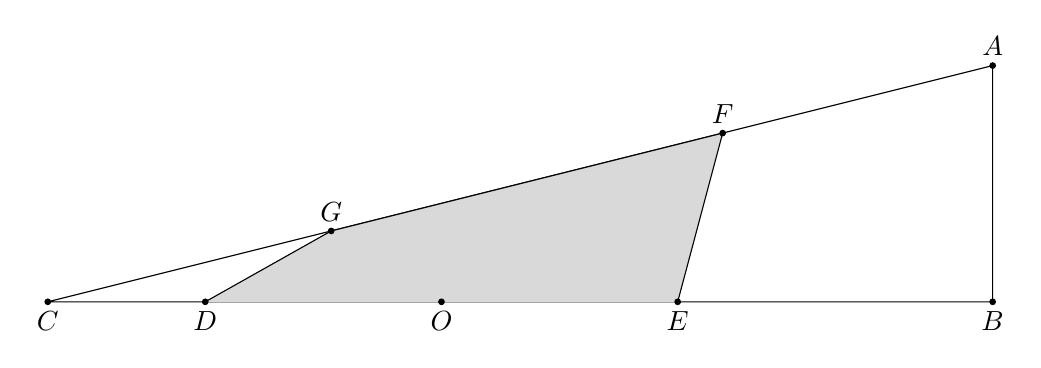
\begin{tikzpicture}

\tkzSetUpPoint[fill=black]
\tkzDefPoint(1, 0){C}
\tkzDefPoint(13,0){B}
\tkzDefPoint(13,3){A}

\tkzDefPoint(6,0){O}
\tkzDefPoint(3,0){D}
\tkzDefPoint(9,0){E}

\tkzDefBarycentricPoint(C=7,A=3)
\tkzGetPoint{G}
\tkzDefBarycentricPoint(C=2,A=5)
\tkzGetPoint{F}

\draw (C) -- (B) -- (A) -- (C);
\draw[fill=gray!30] (D) -- (G) -- (F) -- (E);

\tkzDrawPoints(A, B, C, O, D, E, G, F)

\tkzLabelPoints[below](B, C, O, D, E)
\tkzLabelPoints[above](A, G, F)

\end{tikzpicture}

Wybierzmy O z definicji szerokości. Możemy założyć, że O jest takim punktem, że możliwe d w definicji szerokości jest maksymalne. Wybierzmy punkty D i E na boku BC odpowiednio w stronę C i B od punktu O, aby $|OD| = \frac{3}{2} d$ oraz $|OB| = \frac{3}{2} d$. Jeśli bok BC jest zbyt krótki, obieramy C lub B odpowiednio. Ponieważ punkt O maksymalizuje szerokość, mamy dwa punkty G i F, że $|DG| \leq d$ oraz $|EF| \leq d$ (jeśli bok BC był zbyt krótki, obieramy C i A odpowiednio). Pokażemy, że punkt O daje dobrą szerokość w wielokącie DEFG. Mamy:

\[ d(O, AB) \geq d(O, A) - d(A, B) = d / 2 \]
\[ d(O, GF) = d(O, AC) = d \]

\noindent
Jeśli $B \neq E$:

\[ d(O, EF) \geq d(O, E) - d(E, F) = d/2 \]

\noindent
Jeśli $C \neq D$:

\[ d(O, DG) \geq d(O, D) - d(D, G) = d/2 \]

Jeśli $C = D$, to $d(O, DG) = d(O, C) \geq d$, natomiast przy $E =B$ używamy odległości O od AB. Niezależnie od przypadku otrzymujemy, że O jest odległy od innych boków o przynajmniej $d/2$. Szacujemy obwód:

\[ |DE| + |EF| + |DG| + |FG| \leq 3d + d + d + (3d + d +d) = 10d \]

\noindent
gdzie $|FG|$ szacujemy poprzez długość ścieżki F, E, D, G. Po przejściu z oznaczenia d na t, otrzymujemy tezę. Zauważmy, iż formalnie grubość może być większa od $d/2$, ale może to tylko poprawić oszacowanie obwodu względem t.

\end{proof}

\begin{lemma}\label{lemma:olshanskii_2}

Przypuśćmy, że w przestrzeni geodezyjnej X mamy trójkąt T o 2-rozmiarze b, ale w X nie ma trójkąta o grubości $2b$. Wtedy dla pewnego $t \geq b$ w X jest sześciokąt P, że grubość P jest $\geq t$, a obwód $\leq 42t + \delta$, gdzie delta dowolne rzeczywiste dodatnie.

\end{lemma}

\begin{proof}

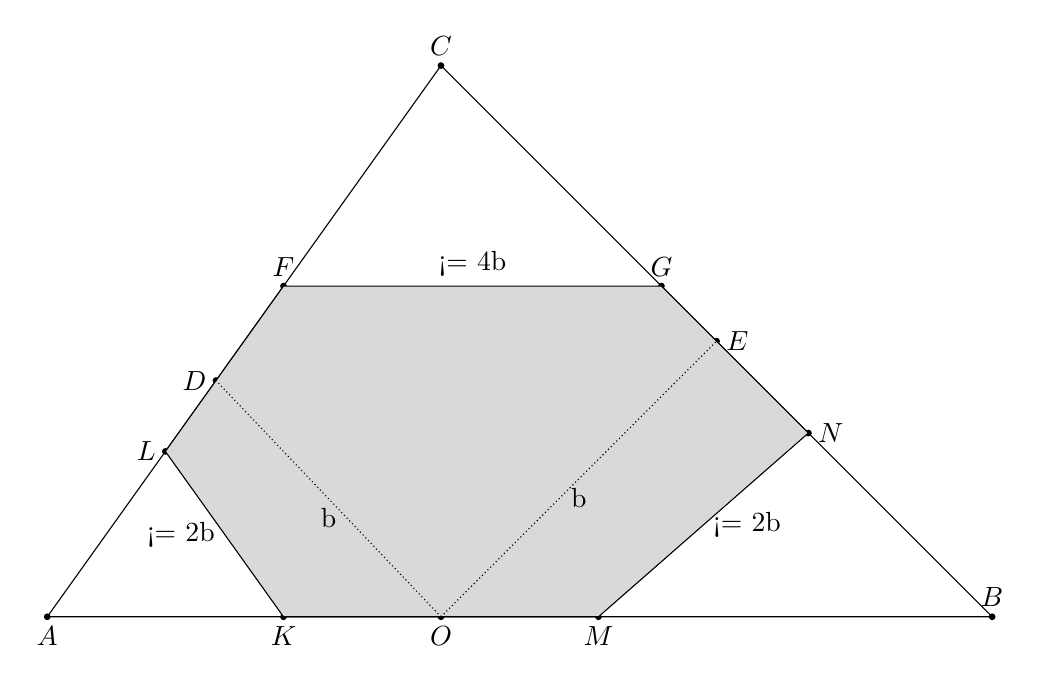
\begin{tikzpicture}

\tkzSetUpPoint[fill=black]
\tkzDefPoint(6, 7){C}
\tkzDefPoint(1,0){A}
\tkzDefPoint(13,0){B}

\tkzDefPoint(6,0){O}
\tkzDefPoint(4,0){K}
\tkzDefPoint(8,0){M}

\tkzDefBarycentricPoint(A=7,C=3)
\tkzGetPoint{L}
\tkzDefBarycentricPoint(B=2,C=1)
\tkzGetPoint{N}

\tkzDefBarycentricPoint(A=4,C=3)
\tkzGetPoint{D}
\tkzDefBarycentricPoint(B=1,C=1)
\tkzGetPoint{E}

\tkzDefBarycentricPoint(A=2,C=3)
\tkzGetPoint{F}
\tkzDefBarycentricPoint(B=2,C=3)
\tkzGetPoint{G}

\tkzDrawPoints(A, B, C, O, D, E, G, F, K, M, N, L)

\draw (A) -- (B) -- (C) -- (A);
\draw[fill=gray!30] (K) -- node[left] {<= 2b} (L) -- (F) -- node[above] {<= 4b} (G) -- (N) -- node[right] {<= 2b} (M) -- (K);

\draw[densely dotted] (O) -- node[below] {b} (D);
\draw[densely dotted] (O) -- node[below] {b} (E);

\tkzLabelPoints[below](A, O, K, M)
\tkzLabelPoints[above](B, G, F, C)
\tkzLabelPoints[left](D, L)
\tkzLabelPoints[right](N, E)

\end{tikzpicture}

Zgodnie z definicją 2-rozmiaru, wybieramy punkt O leżący na boku AB (bez straty ogólności rozważań). Niech D i E to będą punktu z definicji 2-rozmiaru, tj. mamy: 

\[ D \in AC, E \in BC, |DO| = b, |EO| = b \]

Wybierzmy punkty K, M, że:

\[ K, M \in |AB|, |KO| = 3b, |MO| = 3b  \]

\noindent
oraz K i M są po różnych stronach O na AB. Jeśli bok AB jest zby krótki, wybieramy A lub B odpowiednio. Zauważmy, że $d(AD, K) \leq 2b$, gdyż innaczej trójkąt AOD byłby 2b-szeroki. Wybierzmy $L \in AD$, że $d(L, K) \leq 2b$. Zauważmy, że $d(O, LK) \geq d(O, K) - d(K, L) \geq b$.

Punkty M, N są analogiczne dla K, L, lecz konstrujemy je po drugiej stronie punktu O, a $N \in BC$.

Wybierzmy teraz punkt F, że $|DF| = 6b + \epsilon$, F leży na boku AC. Ponieważ $d(D, E) \leq d(D, O) + d(E, O) = 2b$, zatem na mocy założenia o szerokości trójkątów, CDE nie może być 4b-szeroki, więc istnieje G na boku CE, że $d(F, G) \leq 4b$. Zauważmy, że:

\[ d(FG, O) \geq d(F, D) - d(D, O) - d(F, G) \geq b + \epsilon \]

Zatem sześciokąt MKLFGN ma grubość przynajmniej b. Oszacujemy jego obwód. Zaczniemy od pomocniczych długości:

\[ d(L, F) \leq d(L, K) + d(K, O) + d(O, D) + d(D, F) \leq 12b + \epsilon \]
\[ d(G, N) \leq d(N, M) + d(M, O) + d(O, D) + d(D, F) + d(F, G) \leq 16b + \epsilon \]
\[ |MK| + |KL| + |LF| + |FG| + |GN| + |NM|  \leq 6b + 2b + (12b + \epsilon) + 4b + (16b + \epsilon) + 2b = 42b + 2 * \epsilon \]

\end{proof}

\begin{lemma}\label{lemma:olshanskii_3}

Przypuśćmy, że 2-rozmiary trójkątów w przestrzeni geodezyjnej X są nieograniczone. Wtedy dla dowolnego $t_{0} > T$ istnieje w X sześciokąt P o grubości $t > t_{0}$ i obwodzie $\leq 42t + \delta$, gdzie $T$ jest ustaloną stałą.

\end{lemma}

\begin{proof}

Jeśli X zawiera trójkąty o szerokości d dla dowolnego d, to z \ref{lemma:olshanskii_1} dostajemy tezę, bo możemy przyjąć dwa boki o długości zero i z czworokąta dostać sześciokąt. Jeśli natomiast szerokości trójkątów są ograniczone, to \ref{lemma:olshanskii_2} daje nam tezę.

\end{proof}

\chapter{Diagramy van Kampena i grafy Cayley}\label{Van Kampen, Cayley}

Teraz możemy przejść do łącznika pomiędzy grupami, ich prezentacjami a przestrzeniami hiperbolicznymi. Będziemy dla prezentacji grupy rozważać grafy Cayley oraz diagramy van Kampena.

Dobrym opisem diagramów van Kampena jest  \cite{bib:the_geometry_of_the_word_problem}[Rozdział 4], natomiast dla grafów Cayley \cite{bib:geometry_of_word_problem_fin_gen_groups}[Część III, rozdział 1]. Przytoczymy definicję grafu Cayley.

\begin{defi}

Niech S będzie zbiorem generatorów dla grupy G. Grafem Cayley G względem S nazwiemy graf, że jego wierzchołkami są elementy grupy, natomiast dla $g_1, g_2 \in G$ mamy skierowaną krawędź  z $g_1$ do $g_2$ wtedy i tylko wtedy, gdy $g_2 = g_1s$ dla pewnego $s \in S$. Każdej krawędzi przypisujemy długość jeden, jako odległość między dwoma punktami przyjmujemy długość najkrótszej ścieżki.

\end{defi}

\begin{defi}

Mówimy, że skończenie generowana grupa G jest hiperboliczna, jeśli jej graf Cayley $\Gamma$ jest przestrzenią hiperboliczną. Okazuje się to niezależne od wyboru zbioru generatorów.

\end{defi}

\begin{defi}

Niech R będzie zbiorem słów, natomiast $R^C$ to zbiór wszystkich cyklicznych przesunięć słów z R.

Diagramem van Kampena dla słowa w nazwiemy skończony skierowany graf planary $\Delta$, że każdej krawędzi odpowiada litera, na brzegu grafu znajduje się słowo w, natomiast na brzegu każdej ściany (ograniczonej spójnej składowej) znajduje się słowo z $R^C$.

Brzegiem diagramu nazwiemy brzeg nieograniczonej spójnej składowej.

\end{defi}

Poniżej przykładowy diagram van Kampena dla słowa $w = aa^{-1}a^{-1}ba^{-1}b^{-1}aa$ oraz prezentacji $< \{ a, b \} | ab = ba, baa = \epsilon >$

\begin{tikzpicture}

\tkzSetUpPoint[fill=black]
\tkzDefPoint(2, 4){O}
\tkzDefPoint(0.5,6){A_1}
\tkzDefPoint(5,2){A_2}
\tkzDefPoint(9.5,-1){A_3}
\tkzDefPoint(11,5){A_4}
\tkzDefPoint(8.75,8){A_5}
\tkzDefPoint(4.7,5){A_6}
\tkzDefPoint(7.55,2){A_7}


\tkzDrawPoints(O, A_1, A_2, A_3, A_4, A_5, A_6, A_7)
\draw [thick, ->] (O) edge node[above] {a} (A_2) (A_2) edge node[below] {b} (A_7) (A_6) edge node[above] {a} (A_7) (O) edge node[above] {b} (A_6);

\draw [thick, ->] (A_6) edge node[left] {b} (A_5) (A_7) edge node[above] {b} (A_4) (A_5) edge node[above] {a} (A_4);

\draw [thick, ->] (A_7) edge node[above] {a} (A_3) (A_3) edge node[below] {a} (A_2);
\draw [thick, ->] (A_6) edge node[above] {a} (A_1) (A_1) edge node[left] {a} (O);


\tkzLabelPoints[below](O, A_2, A_3)
\tkzLabelPoints[right](A_4)
\tkzLabelPoints[above](A_1, A_6, A_5, A_7)

\end{tikzpicture}


Możemy na wierzchołkach diagramu zdefiniować metrykę, jako długość najkrótszej ścieżki w grafie. Grubość diagramu van Kampena definiuje się analogicznie do grubości wielokąta w przestrzeni metrycznej, ograniczamy tylko zbiór interesujących nas punktów do wierzchołków grafu.

Najważniejszy dla nas będzie lemat van Kampena, dzięki któremu na podstawie lematu \ref{lemma:olshanskii_3} dostaniemy odpowiednio gruby diagram.

\begin{lemma}[van Kampena]

Słowo w spełnia $w \equiv \epsilon$ wtedy i tylko wtedy, gdy istnieje diagram $\Delta$, że w jest jego brzegiem.

\end{lemma}

\begin{lemma}\label{lemma:olshanskii_4}

Przypuśćmy, że 2-rozmiary trójkątów w grafie Cayley'a $\Gamma$ grupy G są nieograniczone. Wtedy dla każdego $t_{0} > 0$ istnieje diagram van Kampena $\Delta$ o grubości $t \geq t_{0}$, a jego średnica jest $\leq 43t$.

\end{lemma}

\begin{proof}

Na podstawie lemat \ref{lemma:olshanskii_3} otrzymujemy w grafie Cayley sześciokąt P o stosownych własnościach (np. $\delta = \frac{1}{2}$).

Z sześciokąta możemy uzyskać wielokąt Q poprzez przesunięcie wierzchołków P do najbliższych wierzchołków grafu Cayley'a. W ten sposób być może zmniejszymy liczbę wierzchołków, gdyż niektóre wierzchołki pokryją się. Możemy oszacować grubość P za pomocą grubości Q:

\[ t(Q) + \frac{1}{2} \geq t(P) \]

\noindent
gdyż dla punktu z P w odległości t(Q) mamy inny bok Q, więc przesuwając się o co najwyżej $\frac{1}{2}$ jeśli trafiliśmy w ten sam bok P, trafimy w inny bok P. Taka transformacja nie zwiększyła też obwodu otrzymanego wielokąta Q.

Z lematu van Kampena, otrzymujemy diagram $\Delta$ o minimalnej liczbie ścian, na którego brzegu mamy słowo z brzegu sześciokąta P. Obierzmy jeden z punktów z brzegu diagramu $\Delta$ i oznaczmy go przez O. Ponieważ możemy w naturalny sposób zanurzyć diagram van Kampena w graf Cayley — przyporządkowujemy wierzchołkom diagramu słowa otrzymane przez przejście ścieżką z punktu O do rozważanego punktu, co jest dobrze zdefiniowane dzięki równoważności każdej pętli i słowa pustego — możemy przenieść własności sześciokąta P na diagram Q. W szczególności, boki diagramu również są geodezyjnymi, gdyż innaczej boki P nie byłby geodezyjnymi. Możemy oszacować grubość wielokąta za pomocą grubości diagramu:

\[ t(\Delta) \geq t(Q) - \frac{1}{2} \]

\noindent
gdyż z każdego punktu Q do pewnego wierzchołka $\Delta$ mamy odległość co najwyżej $\frac{1}{2}$, a od tego punktu w odległości $t(\Delta)$ punkt z innego boku — szacuje to $t(Q)$ z góry.

Zatem dla $t_{0} \geq 42.5$:

\[ |\partial \Delta| = \sum q_{i} \leq \sum p_{i} \leq 42.5t(P) \leq 42.5(t(\Delta) + 1) \leq 43 t(\Delta) \]

\end{proof}

Ten lemat kończy serię technicznych lematów. Ich główną treścią jest stwierdzenie, że jeśli przestrzeń nie jest hiperboliczna, to wielokąty w niej zawarte mogą być grube. Diagramy Van Kampena służą nam jako wygodne narzędzie do pracowania z przestrzeniami metrycznymi otrzymywanymi z grup.

Co bardzo istotne, wspomniane boki diagramu nie są bokami pojedynczych ścianek. Intuicyjnie, otrzymany diagram posiada na brzegu długie fragmenty geodezyjnych.

\chapter{Funkcje Dehan grup hiperbolicznych}\label{Main proof}

Posiadamy już wszystkie narzędzia do wykazania, że grupa jest hiperboliczna tylko wtedy gdy ma liniową funkcję Dehna. Zaprezentujemy dowód w dwie strony. Zaczniemy od prostszej implikacji.

\section{Grupy hiperboliczne posiadają prezentację Dehna}

\begin{ther}\label{thm:hiper_linear}

Każda grupa hiperboliczna posiada prezentację Dehna.

\end{ther}

\begin{proof}[Dowód \ref{thm:hiper_linear}]

Przypomnijmy \ref{thm:dehn_pres_linear}, iż posiadanie prezentacji Dehna implikuje liniowość funkcji Dehna. Będziemy więc dowodzić istnienia prezentacji Dehna dla grup hiperbolicznych. Skorzystamy z Twierdzenia \ref{thm:local_geodesic_is_quasi}. Popatrzmy na graf Cayley'a G - $\Gamma$ jako na przestrzeń hiperboliczną.

Wybieramy $\lambda$ z tego twierdzenia oraz zbiór skończony:

\[ P = \{u \in F(A) : |u| \leq 8 \delta \cdot  max \{1, \lambda \}, \quad \exists v. (|v| < |u| \land u =_{\Gamma} v)  \} \]

\begin{tikzpicture}

\tkzSetUpPoint[fill=black]
\tkzDefPoint(0, 0){O}
\tkzDefPoint(-2,1){A_1}
\tkzDefPoint(-1,5){A_2}
\tkzDefPoint(1.5,6){A_3}
\tkzDefPoint(5,5.5){A_4}
\tkzDefPoint(6,3.5){A_5}
\tkzDefPoint(2,0){A_6}


\tkzDrawPoints(O, A_1, A_2, A_3, A_4, A_5, A_6)
\draw (O) -- (A_1) -- (A_2) -- (A_3) -- (A_4) -- (A_5) -- (A_6) -- (O);
\draw[dotted] (A_3) -- (A_5);


\tkzLabelPoints[below](O, A_6)
\tkzLabelPoints[left](A_1)
\tkzLabelPoints[right](A_5)
\tkzLabelPoints[above](A_2, A_3, A_4)

% title
\node[align=center,font=\bfseries, yshift=2em] (title) 
    at (current bounding box.north)
    {Skracanie pętli w grafie Cayley};

\end{tikzpicture}

Pokażemy, że jest to prezentacja grupy G — dokładniej wszystkie słowa postaci $vu^{-1}$ dla u i v jak powyżej. Weźmy słowo w, $w =_{\Gamma} \epsilon$. Określa ono pewną pętlę $\gamma$ w grafie Cayley'a. Jeśli nie jest to $8 \delta$ - lokalnie geodezyjna, to możemy pewną część ścieżki zastąpić krótszą, tworząc krótsze słowo odpowiadające ścieżce, a znajduje się ono w zbiorze P. Jeśli nie możemy tak zrobić, to na mocy twierdzenia \ref{thm:local_geodesic_is_quasi}, $\gamma$ jest quasi geodezyjną. Zatem możemy napisać:

\[ \frac{|w|}{\lambda} - \eta \leq d_{\Gamma}(\gamma(0), \gamma(1)) \]

\noindent
co po podstawieniu $\gamma(1) = \gamma(0)$, ponieważ mamy pętlę, daje:

\[ |w| \leq \lambda \eta < 8 \lambda \delta \]

\noindent
co w szczególności oznacza, że w jest równoważne $\epsilon$ tylko gdy jest w P.

Zatem dowolne słowo równoważne słowu pustemu można przedstawić za pomocą zbioru  

\[ \{ uv^{-1} : u \in P, \ |v| \leq |u|, uv^{-1} \equiv \epsilon \} \]

\noindent
czyli jest to zbiór relatorów prezentacji grupy G.

\end{proof}

\section{Grupy z podkwadratową funkcją Dehna są hiperboliczne}

Teraz pokażemy, że gdy funkcja Dehna grupy G jest $o(n^2)$, to G jest hiperboliczna.

\begin{ther}\label{thm:subquadratic_hyperbolic}

Jeśli funkcja Dehna grupy G jest $o(n^2)$, to G jest hiperboliczna, a jej funkcja Dehna liniowa.

\end{ther}

Warto przed dowodem podać pewne intuicje.

Kluczowym pomysł jest podany w lemacie poniżej. Wybierzmy punkt z brzegu "grubego" diagramu van Kampena. Popatrzmy na ścianki zawierające ten punkt i przylegające do długiego fragmentu boku diagramu. Następnie na ścianki stykające się z tymi ściankami. Potem na kolejny poziom. Zewnętrzny brzeg doklejonych ścianek będzie się systematycznie wydłużał, a z nim ilość ścianek, tj. relatorów w słowie. Ponieważ długość krawędzi zbioru ścianek będzie przyrastała liniowo, to całkowita ilość ścianek powinna rosnąć z kwadratem długości. Ten heurystyczny sposób myślenia załamuje się, gdy trafimy na zewnętrzny brzeg diagramu. Dlatego tym rozumowaniem możemy uzyskać kwadratową ilość ścianek względem odległości centralnego punktu od reszty brzegu. Potrzebujemy więc wielokąta, którego grubość zależy liniowo od obwodu. Uzyskaniem takiego wielokąta zajmuje się lemat \ref{lemma:olshanskii_4}.

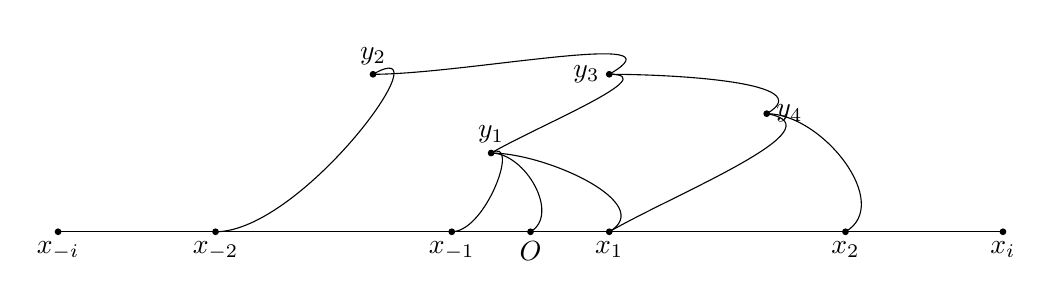
\begin{tikzpicture}

\tkzSetUpPoint[fill=black]

\tkzDefPoint(0, 0){x_{-i}}
\tkzDefPoint(6,0){O}
\tkzDefPoint(12,0){x_i}
\tkzDefPoint(5,0){x_{-1}}
\tkzDefPoint(2,0){x_{-2}}
\tkzDefPoint(7,0){x_{1}}
\tkzDefPoint(10,0){x_{2}}
\tkzDefPoint(5.5,1){y_{1}}
\tkzDefPoint(4,2){y_{2}}
\tkzDefPoint(7,2){y_{3}}
\tkzDefPoint(9,1.5){y_{4}}

\draw  (x_{-i}) -- (O) -- (x_i);
\draw  (x_{-1}) to[out=0,in=+30] (y_{1});
\draw  (y_{1}) to[out=0,in=+30] (O);
\draw  (y_{1}) to[out=0,in=+30] (x_{1});
\draw  (x_{-2}) to[out=0,in=+30] (y_{2});
\draw  (y_{2}) to[out=0,in=+30] (y_{3});
\draw  (y_{3}) to[out=0,in=+30] (y_{1});
\draw  (y_{3}) to[out=0,in=+30] (y_{4});
\draw  (y_{4}) to[out=0,in=+30] (x_{2});
\draw  (y_{4}) to[out=-10,in=+30] (x_{1});

\tkzLabelPoints[below](O)  
\tkzLabelPoints[below](x_i)
\tkzLabelPoints[below](x_{-i}) 
\tkzLabelPoints[below](x_{1})
\tkzLabelPoints[below](x_{-1})
\tkzLabelPoints[below](x_{2})
\tkzLabelPoints[below](x_{-2})

\tkzLabelPoints[above](y_{1})
\tkzLabelPoints[above](y_{2})
\tkzLabelPoints[left](y_{3})
\tkzLabelPoints[right](y_{4})

\tkzDrawPoints(O, x_{-i}, x_i, x_{1}, x_{2}, y_{1}, y_{2},
y_{3}, y_{4}, x_{-1}, x_{-2})

\end{tikzpicture}  

\begin{proof}[Dowód \ref{thm:subquadratic_hyperbolic}]

\begin{lemma}\label{lemma:olshanskii_5}

Ustalmy prezentację grupy G z relatorami $\{ r_{i} \}$, przez M oznaczmy $max(|r_{1}|, ..., |r_{n}|)$. 
Niech $t > 1$ będzie grubością diagramu $\Delta$ z brzegiem $q=q_{1}...q_{n}$. Wtedy ilość ścian m jest taka, że
\[ m \geq (2t/M - 1) ^2 \]

\end{lemma}

\begin{proof}

Będziemy wielokrotnie korzystać z prostego faktu, iż geodezyjne nie zawierają pętli.

Z definicji grubości, możemy wybrać punkt O leżący na boku p brzegu diagramu $\Delta$, że dla każdego wierzchołka  A, $ A \in \partial \Delta, \ A \notin p$, $d(A, O) \geq t$.

Będziemy definiować kolejne zbiory ściany. Przez $F_{0}$ oznaczymy zbiór ścian diagramu zawierające O. Przez $F_{i}$ będziemy oznaczać zbiór tych ścian, które posiadają punkt wspólny ze ścianą należącą do rodziny $F_{j}$ dla $j < i$ oraz nie należą do żadnej z rodzin $F_{j}$ dla $j < i$.

Można o wybieranych ścianach myśleć jak o poziomach ścian otaczających centralny punkt O. Zdefiniujmy $S_{i} \defeq \cup_{k \leq i} F_{k}$. Zbiory $S_{i}$ są spójne i ograniczone. Popatrzmy na ich brzeg, $z_{i}$. Ponieważ punkt O leży na brzegu diagramu $\Delta$, leży także na brzegu każdego ze zbiorów $S_{i}$. W związku z tym możemy przedstawić
\[ z_{i} \defeq x_{i} y_{i} \]
gdzie $y_{i}$ jest najdłuższą ścieżką, że $O \in x_{i}$, a $y_{i} \cap p = \emptyset$. $y_i$ nie jest puste, gdyż gdyby przypuszczając przeciwnie było puste, to mielibyśmy sytuację, w której w otoczeniu O diagram $\Delta$ byłby geodezyjną:

\begin{tikzpicture}

\tkzSetUpPoint[fill=black]
\tkzDefPoint(3, 0){p_{-i}}
\tkzDefPoint(6,0){O}
\tkzDefPoint(10,0){p_i}

\tkzDefPoint(11,1){a}
\tkzDefPoint(11,-1){b}
\tkzDefPoint(2,1){c}
\tkzDefPoint(2,-1){d}

\tkzDrawPoints(a, b, c, d, p_i, p_{-i}, O)

\draw  (p_{-i}) -- (O) -- (p_i);
\draw  (p_i) to[out=0,in=-30] (a);
\draw  (p_i) to[out=0,in=+30] (b);
\draw  (p_{-i}) to[out=-30,in=0] (c);
\draw  (p_{-i}) to[out=-30,in=0] (d);

\tkzLabelPoints[below](O)  
\tkzLabelPoints[above](a)
\tkzLabelPoints[below](b) 

\tkzLabelPoints[above](c)
\tkzLabelPoints[below](d) 
 
\end{tikzpicture}

\noindent
gdzie O i wszystkie ścianki zawierające O leżałyby na p. Zacznijmy od obserwacji, że usuniecie O rozspójniłoby diagram. Gdyby tak nie było, to mielibyśmy w diagramie pętlę zawierającą O (dwóch sąsiadów O na boku p możnaby połączyć ścieżką nie przechodzącą przez O), która musiałaby być zawarta w p (jeśli ścianka objęta pętlą nie zawiera O, to usuwamy ją bez szkody dla istnienia pętli), co jest sprzeczne z geodezyjnością. 

Zatem ponieważ O leży tylko na boku p, podczas przechodzenia po brzegu wzdłuż p musielibyśmy dwa razy przejść przez O, gdyż nie ma innej drogi pomiędzy dwiema składowymi. Daje to znowu pętlę zawartą w p, sprzeczność.

Zauważmy, że dzięki grubości diagramu, do żadnego ze zbiorów $S_{i}$ dla $i + 1 \leq 2t /(M)$ nie należą punkty z $\partial \Delta$ oprócz punktów z boku p. Istotnie, dla każdego punktu ze zbioru $F_{i}$ mamy w odległości co najwyżej $M/2$ wierzchołek ze zbioru $F_{i-1}$ - szacujemy z góry połowę obwodu. Zatem dla dowolnego wierzchołka $A \in F_{i}$ mamy $d(A, O) \leq (i + 1) M / 2$. 

Ograniczymy się do takich niedużych i, tj. $i + 1 \leq \floor{2t / M}$.

Zauważmy, że dwa skrajne wierzchołki $x_i$ leżą na boku p. Gdyby nie leżały, a pomiędzy nimi na tej stronie $z_i$ na której O nie leży był punkt z p, to $y_i$ zawierałoby punkt z p. Gdyby pomiędzy nimi nie było żadnego punktu z p, ponownie w tej części w której nie ma O, to $y_i$ możnaby wydłużyć, wbrew jego definicji. Oznaczmy je przez $p_{-i}$ oraz $p_i$. Przy tych oznaczeniach, dla $t > 1$, $p_{-0} \neq p_0$.

Udowodnimy trzy proste stwierdzenia:

\begin{itemize}

\item $|p_{-i}p_{i}| \geq 2(i + 1)$
\item $y_{i} \cap y_{j} \ = \ \emptyset$ dla $i \neq j$
\item $|y_{i}| \geq 2(i+1)$

\end{itemize}

Dla pierwszego z nich zauważmy, iż $|p_{-0}p_{0}| \geq 2$. Pozostaje teraz spostrzec, że dzięki grubości diagramu, skrajne wierzchołki $p_{\pm i}$ należą do pewnych ścianek, które posiadają bok zawarty w p i nie należą do $S_i$. Zatem w kolejne warstwie dostajemy dwa punkty. Punkty te są różne, gdyż innaczej p zawierałoby pętlę, a jest geodezyjną. Zatem $x_i$ zawiera przynajmniej $2(i + 1) + 1$ różnych punktów z geodezyjnej p (razem z O), w odległości przynajmniej jeden od siebie każdy, więc $|p_{-i}p_{i}| \geq 2(i + 1)$

Przechodząc do drugiego stwierdzenia, gdyby $y_{i} \cap y_{j} \neq \emptyset$, to w szczególności (przypuśćmy $i > j$) oznaczałoby to, że krawędź diagramu v należąca do $y_j \cap y_{i}$ należy do $\partial \Delta$. Uzasadnimy to, przypuśćmy przeciwnie.

Ponieważ $v \in S_j$, więc w $S_j$ jest jedna ścianka, do której v należy. Istnieją co najwyżej dwie ścianki, do których v należy, więc już w $S_{j+1}$ v byłoby krawędzią wewnętrzną. $S_i$ tylko się powiększają, więc v nigdy już nie będzie należało do $z_i$ ani do $y_i$, sprzeczność.

Jeśli krawędź należy do brzegu diagramu, to na mocy założenia o grubość diagramu i liczbie warstw, do których się ograniczyliśmy, oznaczałoby to, że $v \in p$. Nie jest to możliwe, gdyż $v \in y_j$, a $y_j \cap p = \emptyset$, sprzeczność. Zatem zbiory $y_i$ są rozłączne.

Dla trzeciego zauważmy, że $y_i$ łączy dwa punkty $p_{-i}, p_{i}$ leżące na geodezyjnej, więc $|y_{i}| \geq |p_{-i}p_{i}| \geq 2(i + 1)$

Z tych stwierdzeń możemy wyciągnąć końcowe wnioski. Ponieważ kolejne brzegi $y_{i}$ zbiorów $S_{i}$ są rozłaczne, do każdego z nich możemy przyporządkować przynajmniej $|y_{i}| / M$ ścian i żadna przypisana ściana się nie powtórzy — każda taka ściana należy zo zbioru $F_{i}$. W związku z tym możemy oszacować z dołu liczbę ścian diagramu:

\[ m \geq \sum_{1 \leq i \leq \floor{2t/M}} 2i/M \geq \frac{1}{M} (2t/M - 1) ^2 \]

\end{proof}

Teraz możemy zakończyć dowód twierdzenia. Przypuśćmy, że grupa G nie jest hiperboliczna, a jej funkcja Dehna, $D(n)$ jest $o(n^2)$. Na mocy \ref{lemma:olshanskii_4} możemy wybrać ciąg słów $w_n$, że grubość diagramu $w_{n+1}$ jest większe o przynajmniej jeden od grubości diagramu $w_{n}$. Oznaczmy grubość $w_n$ przez $t_n$, wtedy również na podstawie lematu $|w_n| \leq 43|t_n|$ oraz:

\[ D(|w_n|) \geq m(w_n) \geq (2t/M - 1) ^2 \geq (\frac{2 |\partial \Delta|}{43M } - 1) ^ 2  = (\frac{2 |w_n|}{43M } - 1) ^ 2 \]

gdzie $m(w_n)$ oznacza ilość ścian w diagramie słowa $w_n$. Po podzieleniu stronami przez $|w_n|^2$ i przejściu do granicy dostajemy sprzeczność z założeniem, że $D(n)$ jest $o(n^2)$, gdyż $|w_n| \geq t_n$, więc długości słów również rozbiegają do $+ \infty$.

Zatem G jest hiperboliczna.

\end{proof}

\chapter{Zbiór izoperymetryczny}

Przedstawione twierdzenia to nieduży fragment większej teorii. Wspomnimy pokrótce o pewnym ciekawym wyniku.

Naturalne wydaje się pytanie, jakie liczby mogą być wykładnikami funkcji Dehna skończenie prezentowanych grup.

\begin{defi}\label{isoperimetric set}

Definiujemy \textit{zbiór izoperymetryczny} jako:

\[ IP \defeq \{ \alpha : n^{\alpha} \ jest \  \simeq do \ \  pewnej \ \ funkcji \ \ Dehna \} \]

\end{defi}

Pokazaliśmy, że $IP \cap (1, 2) = \emptyset$. Z definicji zbioru \textit{IP} wynika, że jest on podzbiorem $[1, \infty)$. Zauważmy, iż ten zbiór może być co najwyżej przeliczalny, gdyż mamy przeliczalnie wiele skończonych prezentacji grup. Powstaje pytanie, czy zbiór IP ma też inne dziury — okazuje się, że nie, gdyż

\[ \overline{IP} = {1} \cup [2, \infty) \]


Dowód tego faktu można znaleźć na przykład tu \cite{bib:geometry_of_word_problem_fin_gen_groups}.

Zbiór izoperymetryczny ma również wiele innych ciekawych własności. Przytaczanie ich dowodu jest poza zakresem tej pracy, ale warto o nich wspomnieć \cite{bib:isoperimetric_set_turing_machines}:

\begin{itemize}

\item Jeśli $\alpha > 4$, $C \geq 1$ i istnieje maszyna Turinga, która oblicza pierwszych m cyfr  $\alpha$ w czasie $\leq C 2^{2^{Cm}}$, to $\alpha \in IP$
\item Jeśli $\alpha \in IP$, to istnieje maszyna Turinga, która oblicza pierwszych m cyfr $\alpha$ w czasie $\leq C2^{2^{2^{Cm}}}$

\end{itemize}


\begin{thebibliography}{99}
\addcontentsline{toc}{chapter}{Bibliografia}

\bibitem{bib:subquadratic_isoperimetric_inequality} A. Yu. Ol'Shanskii. 
\textit{Hyperbolicity of groups with subquadratic isoperimetric inequality}. 
International Journal of Algebra and Computation, volume 1, issue 3 (1991), DOI: 10.1142/s0218196791000183.

\bibitem{bib:geometry_of_word_problem_fin_gen_groups} Noel Brady, Tim Riley, Hamish Short. 
\textit{The geometry of the Word Problem for Finitely Generated Groups}. 
ISBN 978-3-7643-7949-0, Birkhäuser Verlag (2000).

\bibitem{bib:isoperimetric_set_turing_machines} M. Sapir, J-C. Birget, E. Rips. 
\textit{Isoperimetric and isodiametric functions of groups}. 
Annals of Mathematics (2), vol 156 (2002), no. 2, pp. 345–466.

\bibitem{bib:hyperbolicity_and_thw_word_problem} George Hyun. 
\textit{Hyperbolicity and the word problem}. 

https://math.uchicago.edu/~may/REU2013/REUPapers/Hyun.pdf

\bibitem{bib:the_geometry_of_the_word_problem} Martin R. Bridson. 
\textit{The geometry of the word problem}.

https://people.maths.ox.ac.uk/bridson/papers/bfs/bfs.pdf

\end{thebibliography}

\end{document}

%%% Local Variables:
%%% mode: latex
%%% TeX-master: t
%%% coding: latin-2
%%% End:
